\documentclass{article}[a4paper]
\usepackage[a4paper, total={6.5in, 9.5in}]{geometry}
\usepackage{charter}
\usepackage{graphicx}
\usepackage{float}
\usepackage{listings}
\usepackage{amsmath}
\usepackage{amssymb}
\usepackage{enumitem}
\usepackage{tabularray}

\lstset{
  language=Python,
  basicstyle=\ttfamily,
  keywordstyle=\color{blue},
  commentstyle=\color{gray},
  stringstyle=\color{red},
  showstringspaces=false,
  breaklines=true
}

\title{
	\huge{\textbf{
		Assignment 01
	}}\\
	\Large{
		Intensity Transformations and Neighborhood Filtering
	}\\
	\phantom{}\\
	\large{
		submitted for
	}\\
	\LARGE{
		\textbf{EN3160 - Image Processing and Machine Vision}
	}\\
	\large{
		Department of Electronic and Telecommunication Engineering
	}
	\\
	\large{University of Moratuwa}
}

\author{
	\textbf{Udugamasooriya P. H. J.}\\
	220658U\\
}

\date{12 August 2025}

\allowdisplaybreaks

\begin{document}

\maketitle

\begin{enumerate}
	\item The given transformation is exactly the identity transformation except in the interval from $50$ to $150$, where, if
	the value of a pixel in the original image is denoted by $x$, and its image under the transformation is denoted by $y$, we have \[
		\dfrac{y - 100}{x - 50} = \dfrac{255 - 100}{150 - 50} = 1.55,
	\] which gives \[
		y = 1.55x + 22.5.
	\] This is implemented in the code by first constructing a vector \lstinline|T| representing the identity transformation and then using 
	\lstinline|T[50:151] = 1.55 * T[50:151] + 22.5| to alter only the required portion of it as desrcibed above.

	The output is as follows;
	\begin{figure}[H]
		\centering
		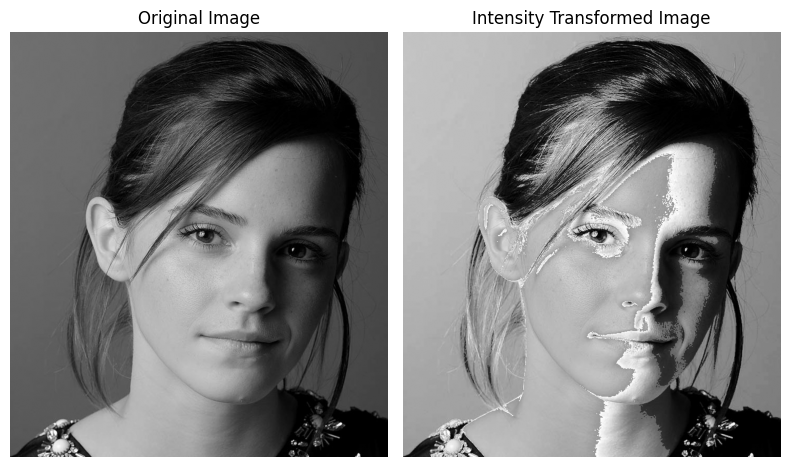
\includegraphics[width=0.7\linewidth]{images/q1.png}
		\caption{Question 1}
	\end{figure}

	\item An eyedropper tool was used to inspect the values of a few representative pixels from the graymatter and whitematter areas and
	it was observed that pixel intensities less than about $175$ correspond to graymatter. To highlight these pixels, we implement the transformation
	given by \[
		\begin{cases}
			x \texttt{ // } 6, & x \leq 175,		\\
			x,		& \text{otherwise},
		\end{cases}
	\] where \texttt{//} denotes the integer-division operation (integer quotient upon division); i.e., we proportionally suppress the 
	intensities of the pixels darker than $175$, and leave the rest unaffected.
	
	A vector denoting this transformation is easily created
	by first creating \lstinline|T| as described above and then executing \lstinline|T[0:175] = T[0:175] // 6|.

	The results are as follows;
	\begin{figure}[H]
		\centering
		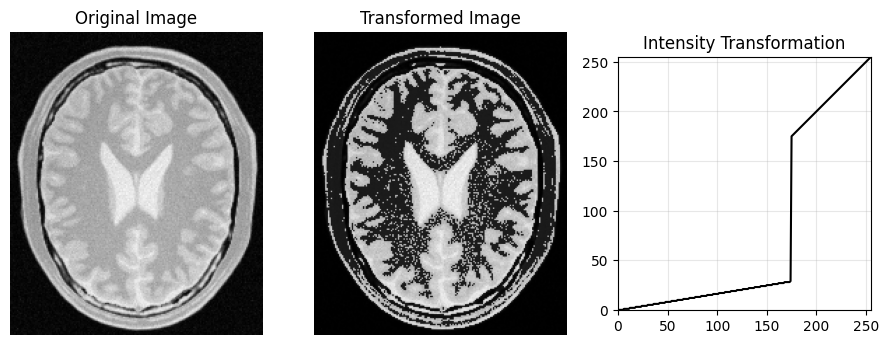
\includegraphics[width=\linewidth]{images/q2.png}
		\caption{Question 2}
	\end{figure}

	\item We open the image, \lstinline|cv2.cvtColor| it from BGR to the LAB color scheme, and extract the L-channel. We then apply the
	gamma transformation specified by \[
		T(x) = 255 \cdot \left(\dfrac{x}{255}\right) ^ \gamma
	\] to the L-channel. The most aesthetically pleasing result was obtained by setting $\gamma = 0.5$. The results are given below.

	\begin{figure}[H]
		\centering
		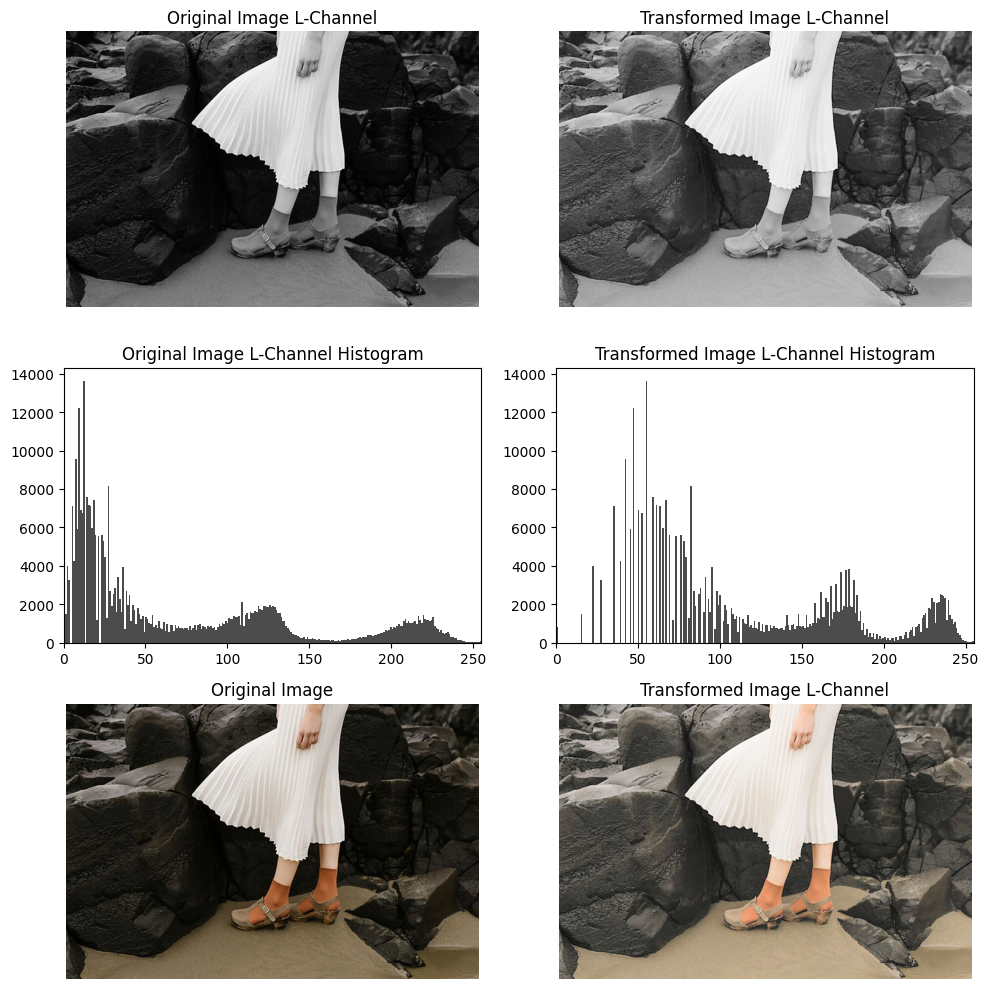
\includegraphics[width=0.9\linewidth]{images/q3.png}
		\caption{Question 3}
	\end{figure}
	
	\item The lines
	\begin{lstlisting}
a = 0.65
sigma = 70

T = np.arange(256, dtype=np.float32)
T = np.minimum(np.ones(256) * 255, T + a * 128 * np.exp(-((T - 128) ** 2) / (2 * sigma ** 2)))
	\end{lstlisting}
	implement the intensity transformation. We provide one vector where all entries are $255$. and another vector populated with entries
	computed according the expression given, and use \lstinline|np.minimum| to pick the smaller of the two. The most aesthetically
	pleasing result was obtained by setting $a = 0.65$. The results are as follows;

	\begin{figure}[H]
		\centering
		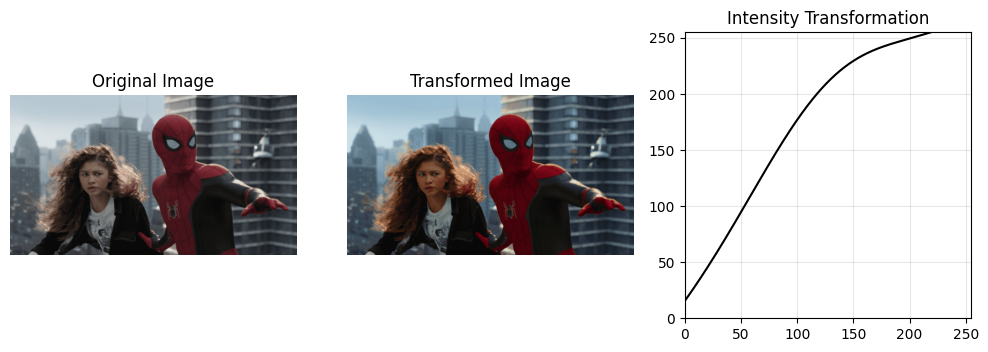
\includegraphics[width=0.9\linewidth]{images/q4.png}
		\caption{Question 4}
	\end{figure}	

\end{enumerate}

\end{document}